\label{chap2}
\section{Information Security}

Information security is the effort to protect information - be it in electronic or physical form - from adversary threats. 
The domain in which the data is to protected can be time, i.e. protecting saved information for later usage, or space, i.e. protect information
transmitted physically from one user to another. To protect information, three key objectives must be met:
\\
\\
\textbf{Confidentiality} is used to protect sensitive information from eavesdroppers who are not allowed to get knowledge of that information.
\\
\textbf{Integrity} ensures that some kind of information can not be altered by third-parties, or that such a modification can be detected by the
receiver of the information, and also includes information non-repudiation. Integrity can be separated into data integrity and system integrity. While the first one assures
that information is only modified in an authorized manner, the latter one demands that a system performs its intended function, free from manipulation.
\\
\textbf{Availability} guarantees that the system works promptly and information, which is needed by an entity to provide some service, is accessible.
\\
\\
Because all three properties go hand-in-hand with each other they are also called the \textit{"CIA - triad"} \cite{stallings} - successfully attacking one property may allow attacking
another one. 
\\
For example, if a
confidentiality attack against a computer system responsible for money transfers can be conducted to steal a password used for controlling this system,
an attacker
can subsequently render the system unusable, therefore compromising availability. On the other hand, the attacker could also try to remain undetected and change
booking orders, thus mounting an attack against the integrity of the system. Thus, these three basic concepts are interleaved and building a system which honors
only parts of them will most likely lead to an insecure system.
\\
In addition to the three objectives listed above, additional security objectives are used frequently: \textbf{authenticity} is the property of being genuine and being able to be 
trusted, while \textbf{accountability} allows to trace the actions of an entity uniquely to that entity.
%Integrity and authenticity are semantically related: checking the integrity implicitly checks authenticity, provided that the key used to generate the tag is only known to authentic entities.
%Vice versa, authenticating the sender of a message is only useful if the message itself cannot be modified by an adversary, i.e. integrity is guaranteed.
%To avoid confusion, the term integrity is used if the meaning is clear from the context.
\subsection{Threats}
Threats form a \textit{potential} violation of security - a violation must not need to occur for there to be a threat. Stallings \cite{stallingsThreat}
divides threat consequences into four categories:
\begin{itemize}
 \item \textbf{Unauthorized disclosure} is a threat aimed against confidentiality. It occurs when an entity gains access to information for which it is not authorized.
 \item \textbf{Deception} threatens system integrity, and may result in tricking an authorized entity into accepting modified data.
 \item \textbf{Usurpation} opposes data integrity s.t. a system is controlled by an unauthorized entity.
  \item \textbf{Disruption} compromises the availability s.t. the system services do not operate correctly.
\end{itemize}

\subsection{Attacks}\label{sec:attacks}
Attacks are the manifestation of a security violation, exploited by an attacker. 
A classification of attacks against communication networks is given in Figure \ref{fig:attacks}.  

\begin{figure}[h]
    \centering
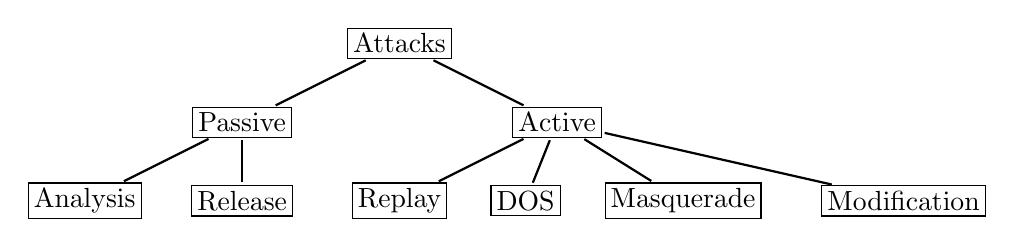
\begin{tikzpicture}[scale=0.2]
\tikzstyle{every node}+=[inner sep=2pt]
\tikzstyle{arrow}=[draw, -latex] 
\tikzset{
    pil/.style={
           ->,
           thick,
           shorten <=1pt,
           shorten >=1pt,}
}
    \node[draw,rectangle] at (10,-5)		(attacks)			{Attacks}; 
    \node[draw,rectangle] at (0,-10)		(passive)			{Passive}; 
     \node[draw,rectangle] at (20,-10)		(active)			{Active}; 
    \node[draw,rectangle] at (0,-15)		(rel)			{Release}; 
    \node[draw,rectangle] at (-10,-15)		(ana)			{Analysis}; 
     \node[draw,rectangle] at (10,-15)		(repl)			{Replay}; 
     \node[draw,rectangle] at (18,-15)		(dos)			{DOS}; 
     \node[draw,rectangle] at (28,-15)		(masq)			{Masquerade}; 
     \node[draw,rectangle] at (42,-15)		(mod)			{Modification}; 

\path[pil,->] (attacks)  (passive); 
\path[pil,-] (attacks)  edge[auto]   node[] {} (passive); 
\path[pil,-] (passive)  edge[auto]   node[] {} (ana); 
\path[pil,-] (passive)  edge[auto]   node[] {} (rel); 
\path[pil,-] (attacks)  edge[auto]   node[] {} (active); 
\path[pil,-] (active)  edge[auto]   node[] {} (dos); 
\path[pil,-] (active)  edge[auto]   node[] {} (repl); 
\path[pil,-] (active)  edge[auto]   node[] {} (masq); 
\path[pil,-] (active)  edge[auto]   node[] {} (mod); 
\end{tikzpicture}
\caption{Classification of attacks}
    \label{fig:attacks}
\end{figure}

% \begin{figure}[h]
%     \centering
%     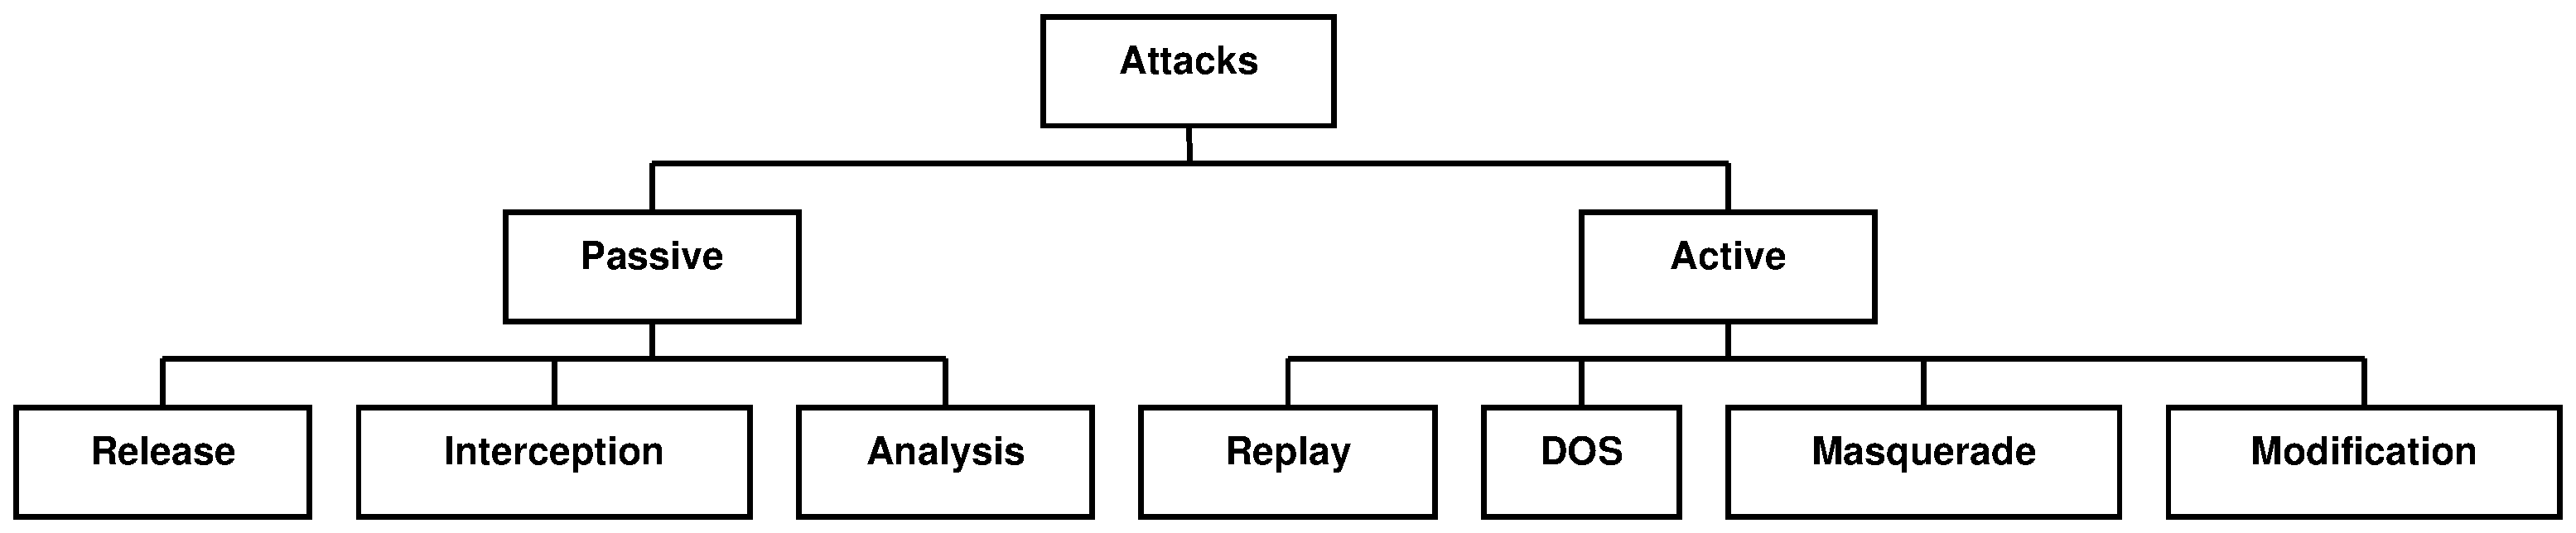
\includegraphics[width=1\textwidth]{figures/attacks.eps}
%     \caption{Classification of attacks}
%     \label{fig:attacks}
% \end{figure}
% The standard model for entity $A$ sending information to entity $B$ is shown in Figure \ref{fig:stdComm}. 
% \begin{figure}[h]
%  \centering
% \begin{tikzpicture}[scale=0.2]
% \tikzstyle{every node}+=[inner sep=2pt]
% \tikzstyle{arrow}=[draw, -latex] 
% \tikzset{
%     pil/.style={
%            ->,
%            thick,
%            shorten <=1pt,
%            shorten >=1pt,}
% }
% \usetikzlibrary{automata,positioning}
% \usetikzlibrary{positioning}
% 
% \node[state,text width=0.8cm,align=center]					at (-40,0)		(a)		{A}; 
% \node[state,text width=0.8cm,align=center]					at (0,0)		(b)		{B}; 
% \path[pil,->] (a)  edge[auto]   node[text width=1cm] {} (b);
% \end{tikzpicture}
% \caption{Communication between two users}
% \label{fig:stdComm}
% \end{figure}
\subsection{Passive attacks}
Passive attacks are aimed against confidentiality. The attacker $E$ intercepts the data transmitted between the two or more entities by monitoring the communication
medium, recording all the traffic. 
\\
After obtaining the data, the attacker can \textbf{release} the data itself to an outside entity. Another way to exploit the data is to \textbf{analyze} them,
allowing the attacker to get knowledge of some kind of meta data like origin, destination, quantity and frequency of the data flows. 
\\
Because of its passive nature the data sent are not modified, thus such an attack is hard to detect. On the other hand, encrypting the traffic to gain confidentiality suffices to guard
against the release of data. To guard against traffic analysis is harder because it may be impossible to encrypt some kind of meta data: for example, the destination address of a
message may not be encrypted because routers handling the message must be able to determine the next routing decision based on this address.
Another reason is that some meta information will always be present, like the size of the message or the simple fact that communication between two points has occurred.
\begin{figure}[h]
\centering
\begin{tikzpicture}[scale=0.2]
\tikzstyle{every node}+=[inner sep=2pt]
\tikzstyle{arrow}=[draw, -latex] 
\tikzset{
    pil/.style={
           ->,
           thick,
           shorten <=1pt,
           shorten >=1pt,}
}
\usetikzlibrary{automata,positioning}
\usetikzlibrary{positioning}
\node[state,text width=0.8cm,align=center]					at (-40,0)		(a)		{A}; 
\node[state,text width=0.8cm,align=center]					at (0,0)		(b)		{B}; 
\node[state,text width=0.8cm,align=center]					at (-20,-10)		(e)		{E}; 
\node[state,text width=0.1cm,align=center,minimum size=0.1,fill]		at (-20,0)		(+)		{}; 
\path[pil,->] (a)  edge[auto]   node[text width=1cm] {} (b);
\path[pil,->] (+)  edge[auto]   node[text width=1cm] {} (e);
\end{tikzpicture}
\label{fig:passAttack}
\caption{Passive attack}
\end{figure}
\subsection{Active attacks}
Unfortunately, a restriction to passive attacks only is no realistic assumption for many systems. Whenever the adversary has access to the communication medium, active attacks
cannot be ruled out, allowing the attacker to modify the data stream, or to create false ones. In contrast to their passive counterparts, active attacks can be detected but
not prevented, so the focus lies on detecting and recovering from active attacks.
\\
\\
\begin{figure}[hf]
\centering
\begin{tikzpicture}[scale=0.2]
\tikzstyle{every node}+=[inner sep=2pt]
\tikzstyle{arrow}=[draw, -latex] 
\tikzset{
    pil/.style={
           ->,
           thick,
           shorten <=1pt,
           shorten >=1pt,}
}
\usetikzlibrary{automata,positioning}
\usetikzlibrary{positioning}
\node[state,text width=0.8cm,align=center]					at (-40,0)		(a)		{A}; 
\node[state,text width=0.8cm,align=center]					at (0,0)		(b)		{B}; 
\node[state,text width=0.8cm,align=center]					at (-20,-10)		(e)		{E}; 
\node[state,text width=0.1cm,align=center,minimum size=0.1,fill]		at (-20,0)		(+)		{}; 
\path[pil,->] (a)  edge[auto]   node[text width=1cm] {} (b);
\path[pil,->] (e)  edge[auto]   node[text width=1cm] {} (+);
\end{tikzpicture}
\label{fig:actAttack}
\caption{Active attack}
\end{figure}
A \textbf{replay} attack consists of two steps: first, the attacker monitors the traffic (i.e. conducts a passive attack) and injects this recorded package in the second step,
thus trying to produce an unauthorized effect.
Of course the package can also be modified and injected afterwards, resulting in a \textbf{modification} attack.
A \textbf{Denial of Service (DOS)} attack tries to overload system resources, attacking availability s.t. the system is not
usable by legitimate users. Finally, \textbf{masquerade} attacks occurs when one entity pretends to be another entity, often based on replay attacks by replying (modified)
authentication messages of an authorized entity.
\\
\\
To prevent active attacks, integrity mechanisms must be combined with confidentiality mechanisms - 
the basic tool to achieve them is cryptography, introduced in the next Section \ref{sec:crypto}. To provide availability, different techniques must be used,
as shown in Section \ref{sec:availability}.

\section{Cryptography}\label{sec:crypto}
Cryptography\footnote{classical greek for \textit{krypt\^{o}s}: \textit{concealed}}
is the science of encrypting information - its evolution was no linear process. Ciphers were used independently in different
places, were forgotten and disappeared when the corresponding civilization died.
A short time table for prominent events is presented below; for a comprehensive outline of cryptographic history, "The Codebreakers", written by David Kahn,
is suggested \cite{codebreakers}.
\\
\\
One of the oldest witnesses for cryptography are hieroglyphs used in Egypt about 2000 B.C., forming the predecessor
of a simple substitution cipher. 500 B.C., the "skytale" was used by greek and spartan military leaders, performing a transposition cipher. Another classical
example was the "Caesar Cipher", named after its inventor and used about 100 B.C. to hide information by replacing every letter of the alphabet by a letter some fixed number down the alphabet,
thus performing a substitution cipher. Ahmas al-Qalqashandi, an egypt writer, introduced the frequency analysis, a method for breaking substitution ciphers,
in the 14th century. About 300 years later, the "Geheime Kabinets-Kanzlei" in Vienna routinely intercepts, copies and 
 re-seales diplomatic correspondence to embassies, and manages to decrypt a great percentage of the ciphertexts. In the beginning of the 20th century, the 
 first cryptographic device called "Enigma"\footnote{classical greek for "riddle"} is patented for commercial use and is later used in World War 2 by german troops for 
 military communication. Successful attacks against the "Enigma" cipher are demonstrated by polish mathematicians even before outbreak of the war, and systematic
 decryption of "Enigma" - based ciphertexts are conducted in Bleatchley Park, U.K., by using so called "Turing-Bombs", giving the allies invaluable advantages.
The second half of the 20th century introduces public key cryptography: in 1976 Whitfield Diffie and Martin Hellman specify a 
protocol for key exchange, based on a public key system developed by Ralph Merkle, and one year later, the RSA public key encryption is found by the american
mathematicians Rivest, Shamir and Adleman.
\\
Cryptography is basically the art of hiding information by turning cleartext
data into a random looking stream or block of bits, called ciphertext, using some kind of
\textit{key}. This process is referred to as \textit{encryption} in general, but it is important to note that for many block ciphers, this encryption process
can also be used to generate a special tag called \gls{mac2}, providing integrity.
\\
The next sections deal with how to achieve confidentiality, the 
concepts how to achieve integrity are partially based on the confidentiality methods and are introduced in Section \ref{Integrity}.
\\
\\
Key, clear- and cipher text all are strings built from the alphabet $\mathcal{A}$. 
\begin{itemize}
 \item $\mathcal{A}$ is a finite set, denoting the alphabet used, for example
 $\mathcal{A} = \{0, 1\}$
 \item $\{0, 1\}^n$ denotes the set of all possible strings with length $n$
 \item $\mathcal{M}$ is the message space, consisting of all strings that can be built with the 
 underlying alphabet
 \item $\mathcal{C}$ is the ciphertext space, also consisting of the strings from 
 the alphbet
$\mathcal{A} = \{0, 1\}$
\item $\mathcal{K}$ is called keyspace, also built from the alphabet. Every element
 $e \in \mathcal{K}$ is called a key and determines the function $\mathcal{M} \rightarrow \mathcal{C}$.
 This function, $E_e$ is called the \textit{encryption function}. 
  \begin{center}
 $ciphertext = E_e(e, cleartext)$
  \end{center}
\end{itemize}
Unauthorized parties - lacking the used key - should, by looking at the ciphertext, learn
absolutely nothing about the hidden cleartext beside the length of the origin message. Authorized parties, on the other hand, are
able to retrieve the original data out of the ciphertext by using the key with polynomial work, thus reversing
the encryption. This reversing process is called \textit{decryption}.
\begin{itemize}
 \item For every key $d \in \mathcal{K}$, $D_d$ denotes the function from $\mathcal{C} \rightarrow
  \mathcal{M}$, and is called \textit{decryption function}.
  \begin{center}
  $cleartext  = D_d(d, ciphertext)$
    \end{center}
\end{itemize}
The keys $e$ and $d$ are also referred to as \textit{keypair}, written $(e,d)$. 
If it is computationally easy to derive the private key $e$ from the public key $d$ (in most cases $e = d$), the encryption scheme
is called \textit{symmetric}, otherwise the scheme is called \textit{asymmetric}.
\\
Combining this properties yields a cipher or \textit{encryption scheme} defined over $\mathcal{(K,M,C)}$, which is a pair of \textit{efficient}
 \footnote{"runs in polynomial time"} algorithms s.t.
 \begin{center}
   $\mathcal{K} \times \mathcal{M} \rightarrow \mathcal{C}$
   \\
   $\mathcal{K} \times \mathcal{C} \rightarrow \mathcal{M}$
 \end{center}
 The correctness property ensures for every pair of $(e,d) \in \mathcal{K}$ and for every message $m \in \mathcal{M}$ that encryption is reverseable, i.e. 
 it must hold that 
 \begin{center}  
 $ m = D_d(d, (E_e(e, m))$
  \end{center}

\subsection{Security of a cipher}

\subsubsection{Perfect secrecy}

A formal definition of a secure cipher was introduced by Shannon in 1949 \cite{6769090}, viewed from a communication-theory point of view, as follows:
given a finite message space, every possible cleartext message has its own \textit{a priori} probability (for example, the distribution of letters in a 
specific language). Additionally, every key can be chosen with specific probability. It is assumed that these
two probabilities constitute the a priori knowledge of an attacker.
\\
A message is picked, encrypted
and sent to the receiver. The eavesdropper, intercepting the message, can calculate the \textit{a posteriori} probabilities for all possible cleartext messages, 
leading to the observed cipher text - these are the conditional properties that under a fixed key, encrypting the cleartext message lead to the
observed ciphertext message.
\\
If the a posteriori probabilities for all possible encryptions are the same as all a priory probabilities, the attacker has learned absolutely
nothing from intercepting the cipher text, which is defined by Shannon as \textit{perfect secrecy}. Such a cipher cannot be broken by a ciphertext-only-attack,
even by an adversary with unlimited time and processing power.
\\
Shannon proofed that for a perfectly secure cipher, the key space must be at least as big as the message space.
Otherwise there will exist cleartext messages which are mapped to the same cipher texts, and thus a priori and a posteriori probabilities will be different,
allowing the attacker to get knowledge he should not have gotten. 

\subsubsection{Semantic security}

Another definition of the security of a cipher, based on complexity theory, is \textit{semantic security}.
To be semantically secure, a cipher must not be breakable by an adversary in a reasonable time
frame \cite{handbook1}, where this time frame is a function of the useful timespan of the protected data. This synonymously means for a semantically secure
cipher that an adversary must be forced to spend super-polynomial time to be able to break it. It follows that \textit{all} semantically secure ciphers
can be broken in principle by mounting the "brute-focrce" attack, searching the correct $n$-bit key in the exponential big key space $2^n$. Thus, such an
exhaustive search must be rendered impracticable by using a suitable large key space to obtain a secure cipher.
Semantic security is therefore a weaker form of security, namely perfect secrecy against an adversary having only polynomially bounded
processing powers \cite{GoldwasserMicali}.

\subsubsection{Kerckhoff's principle}
When designing cryptographic systems, a fundamental question is what components of it must be protected from public knowledge, and what parts can be
published without compromising the security of the system. 
\\
The dutch cryptographer Auguste Kerckhoff stated rules for designing a secure cipher.
According to \textit{Kerckhoff's Principle} stated in the year 1883, among other properties, a secure system should not rely on the secrecy of
its components, the only part that should be kept secret is the key alone. Shannon acknowledged these assumptions to be "pessimistic and hence safe, but 
in the long run realistic, since one must expect the system to be found out eventually".
\\
\\
Mapped to the definitions above, the sets $\mathcal{M, C, K}$, as well as the
transformation functions $E_e$ and $D_d$, must not be secret. The only thing that has to be kept private is the decryption key $d$.
This separation of key and algorithm allows the publication of the basic cipher methods, benefiting from peer review. A contradicting approach 
trying to strengthen the safety of a cryptographic system by hiding the inner workings of it from public is also known as "Security by Obscurity".

\subsection{Randomness and Probabilistic Theory}
A basic requirement of all cryptographic schemes is the availability of randomness. \textit{Entropy}, denoted $H$, is the unit of the unpredictability of a process, as
 defined by Shannon in \cite{6773024}:
 \begin{align}
 H(X) = - \sum_{x \in X}^{} p(x) * ln(p(x))
\end{align}
The higher the predictability, or in other words, the more likely an event, the lower its entropy. Flipping a "fair" coin is a canonical 
example of a process with maximum entropy, because every coin flip has a probability of $\frac{1}{2}$, and all flips are independent from each other \cite{1621063}.
If obtaining heads of the coin is viewed as a logical "0" and tails as a logical "1", a binary string of length $n$ can be built, where the probability of all possible
strings of same length is equal, as shown in Figure \ref{fig:uniform}, yielding an \textit{uniform distribution}, with
$H = 2^n*\frac{1}{2^n}*ln(2^n) = n$ bit. 
\\
\\
The importance of random numbers in cryptography is founded on the nature of the cipher used, as will be shown in the next sections. For example
stream ciphers generate a keystream which is used
for encryption. If the keystream is predictable by an adversary, the security of the cipher is reduced. Similar arguments are valid for block ciphers, which often
rely on an initial value called \gls{iv} for encryption. Also, many key negotiation algorithms schemes rely on determining a random prime number, which is often 
achieved by choosing a random number and testing it for primality. Again, if such a prime number can be narrowed down within some boarders, this fact may
weaken the encryption process.
\\
A fundamental problem in generating random numbers by utilizing computing devices is the deterministic nature of an algorithm:
\\
\\
\textit{"Anyone who considers arithmetical methods of producing random digits is, of course, in a state of sin."} \footnote{John von Neumann, 1951}
\\
\\
Such numbers are therefore called \textit{pseudo}random. Lots of cryptographic products suffered serious flaws because of relying on a broken \gls{prng}. A 
historical example of such a broken random number generator, outputting biased (i.e. not uniformly distributed) values was "RANDU", invented by IBM in the
1960s. 
The generator belongs to the class of multiplicative congruential algorithms as proposed by Lehmer \cite{MR0044899}, which can in principle generate random
numbers of sufficient quality, \textbf{if} the parameters are chosen correctly.
Random values can be obtained after setting an initial value for $I_0$, called \textit{seed}, and repeatedly executing the calculation
\begin{center}
 $I_{j+1} = 65539 * I_j \pmod{2^{31}}$		% FIXME: unvollendeter satz...?
\end{center}
One problem 
is that consecutive values generated by RANDU are not independent, a fact that	 can be seen in Figure \ref{fig:randu}. To obtain the plot, 10000 uniformly distributed 
random numbers were chosen as initial seeds for $I_i$ and plotted as x-values, $I_{i+1}$ served as y- and $I_{i+2}$ as z-values. While one would suspect that all points
would be equally distributed in space, a clear pattern is visible, indicating that the values are correlated.
\\
To assess the quality of a \gls{prng}, beside of such spectral tests lots of additional tests are available, see \cite{nistRAND} for details.
\\
To encounter the shortcomings of a \gls{prng}, a \gls{trng} uses a natural process as non-deterministic data source, for example
thermal noise of a semi conductor, cosmic noise from space or digital oscillators.
\begin{figure}
    \centering
    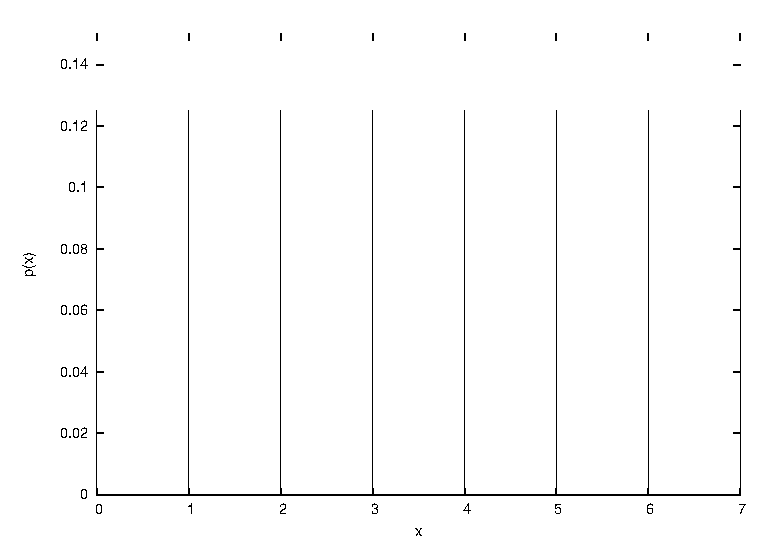
\includegraphics[width=0.6\textwidth]{figures/uniform}
    \caption{Uniform Distribution of binary string of length three}
    \label{fig:uniform}
\end{figure}
\begin{figure}
    \centering
    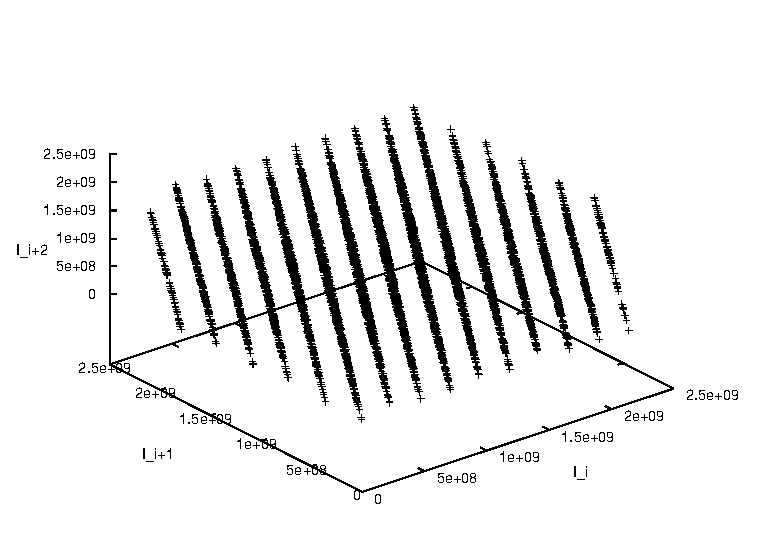
\includegraphics[width=1\textwidth]{figures/randu}
    \caption{Spectral Plot of RANDU output}
    \label{fig:randu}
\end{figure}

\subsection{The discrete logarithm problem}\label{refDLP}
The \gls{dlp}, a mathematical problem, is the basis of two important key exchange algorithms, both introduced in Section \ref{pkc}: the first one, \gls{dh} utilizes finite fields, whose
theoretical background is introduced below. \glspl{ec}, basis for the second algorithm, are also explained.

\subsubsection{Finite Fields \gls{dlp}}
A field consists of a set $\mathcal{F}$ together with two operations $\cdot$, namely addition "+" and multiplication "*", satisfying the following properties:
\begin{itemize}
 \item  Closure: for all elements from $\mathcal{F}$, the set is closed under the defined operations, i.e. applying an operator $\cdot$ to two elements from the set results in an
element also belonging to the set.
 \item Associativity and commutativity hold, i.e. $a \cdot (b \cdot c) = (a \cdot b) \cdot c$ and $a \cdot b = b \cdot a$
 \item For both operations and all elements from the set $\mathcal{F}$ an identity element $e$ exists s.t. $a\cdot e = a$
 \item For both operations and all elements from the set $\mathcal{F} \backslash \{0\}$ an inverse element exists s.t. $a\cdot a^{-1} = e$
 \item Distributivity holds: $(a+b) \cdot c = a \cdot c + b \cdot c$ for all elements 
\end{itemize}
For a finite field, the size of the set 
$\mathcal{F}$ is finite and called \textit{order} of the field, with neutral elements for addition and
multiplication. Inverses can be found to for all
elements regarding addition s.t. $a + (-a) = e$ and regarding multiplication for all elements except ${0}$ s.t. $a * a^{-1} = e$.
\\
\\
A specific example of a finite field is a prime file, which can be constructed by taking the set of integers $\mathbb{Z}\pmod p$, with $p \in \mathbb{P}$, thus
restricting the set of all integers to the set $\mathbb{Z}_p = \{0, 1, ..., p-1\}$.
By choosing $p$ as prime it is ensured that for any element $a \in \mathcal{F} \backslash\{0\}$, a multiplicative inverse exists: $ a * a^{-1} = 1 \pmod p$.
The set of numbers for which multiplicative inverses exist is called $\mathbb{Z}{_p}^*$, so for $p$ being prime, $\mathbb{Z}_p \backslash \{0\} = \mathbb{Z}{_p}^*$.
\\
By raising an element $a \in \mathbb{Z}_p$ to different powers, a subgroup of $\mathbb{Z}{_p}^*$
is generated, a fact that follows from Fermat's little theorem stating that for $p$ being prime and raising $a$ to the power $p-1$, the outcome is congruent 1
modulo p:
\begin{center}
 $a^{p-1} \equiv 1 \pmod p $ \\
\end{center}
Raising $a$ to higher powers results in:
\begin{center}
 $a^{p} \equiv a*a^{p-1} \equiv a \pmod p$ \\
 $...$ \\
 $a^{2p} \equiv a^2 * a^{p-1} * a^{p-1} \equiv a^2 \pmod p$
\end{center}
Thus, generating higher powers than $(p-1)$ does not yield different outcomes. If by raising $a$ to $(p-1)$ different powers all elements from $\mathbb{Z}{_p}^*$ can
be generated, $a$ is called \textit{primitive root} or \textit{generator}, generating a cyclic group.
If $p$ is prime it can be shown that at least one such generator $g$ must exist and can be found efficiently \cite{primitiveRoot}.
Conversely this means that for all elements from  $\mathbb{Z}{_p}^*$ a unique exponent in the interval $[0, p-1]$ exists,
called the \textit{discrete logarithm for the base $ g \pmod p$}.
\\
\\
To find
the discrete logarithm, several algorithms exist. The most naive method conducts an exhaustive search, so for a prime of $n$ bits length, $2^n$ search operations
are necessary. More efficient algorithms exist, with the best methods finishing after about $2^{\frac{n}{2}}$ steps \cite{5199978}. 
Therefore, by choosing a sufficient large prime, finding the discrete logarithm is considered a hard problem, a fact
that is exploited by the \gls{dh} key exchange algorithm and its variants.

\subsubsection{Elliptic curve \gls{dlp}}\label{sec:ecIntro}
An \gls{ec} is basically the set of all points
satisfying an equation with the form as shown in \ref{basicEC}, called "Weierstraß" equation:

\begin{align}\label{basicEC}
 y^2 = x^3 + ax +b
\end{align}
The additional condition $4a^3 + 27b^3 \neq 0$ assures that the \gls{ec} does not possess any singularities.
\\
An imaginary point "in infinity", denoted $\infty$, serves as additive neutral element, and also belongs to the \gls{ec} by definition:
\begin{center}
 $P + \infty = \infty + P = P, P + (-P) = \infty$
\end{center}
Negatives can be calculated easily due to the symmetric nature of the curves by swapping the sign of the y-coordinate of the point. For point $P$ with coordinates $(x, y)$, $-P$ is defined as
$(x,-y)$, thus satisfying $P + (-P) = \infty$.
\\
By defining an \gls{ec} over $\mathbb{Z}_p$, with $a, b \in \mathbb{Z}_p$, a cyclic group can be generated. The addition operation that "adds" two points on
this curve is defined by a "chord-and-tangent" rule. Figure \ref{fig:ecAdd}
shows addition of two points, while \ref{fig:ecDouble} shows adding a point to itself. It is important to note that this representation is shown in the domain
$\mathbb{R}$ for visualization - in real \gls{ec} cryptography, only elements $\pmod p$ (i.e. from the set $\mathbb{Z}_p$)
are allowed to avoid rounding errors. 
\\
\\
Addition is defined as connecting points $A$ and 
$Q$, finding the intersection of the line with the \gls{ec} ($R'$) and reflecting that point across the x-axis to obtain the result $R$. 
%\begin{minipage}{\linewidth}
%      \centering
%      \begin{minipage}{0.8\linewidth}
          \begin{figure}[H]
          \centering
              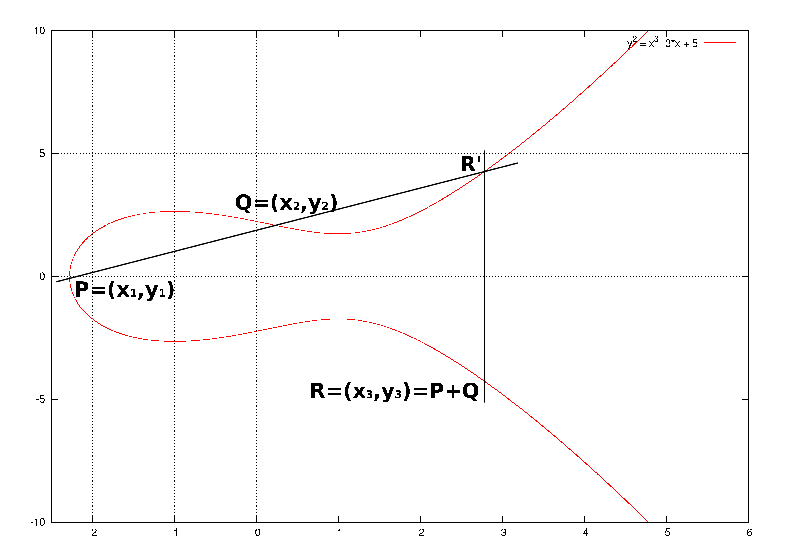
\includegraphics[width=0.6\linewidth]{figures/ecAdd.eps}
              \caption{Adding two points}
              \label{fig:ecAdd}
          \end{figure}
Mathematically, the new coordinates can be calculated as shown in equation \ref{adding}:
\begin{align}\label{adding}
x_3 = (\frac{y_2-y_1}{x_2-x_1})^2-x_1-x_2, y_3=\frac{y_2-y_1}{x_2-x_1}(x_1-x_3)-y_1
\end{align}   
Point-doubling of $P$ is achieved in a similar way by determining the tangent of $P$, finding the intersection and reflection.
%      \end{minipage}
     % \hspace{0.05\linewidth}
%      \begin{minipage}{0.8\linewidth}
          \begin{figure}[H]
	    \centering
              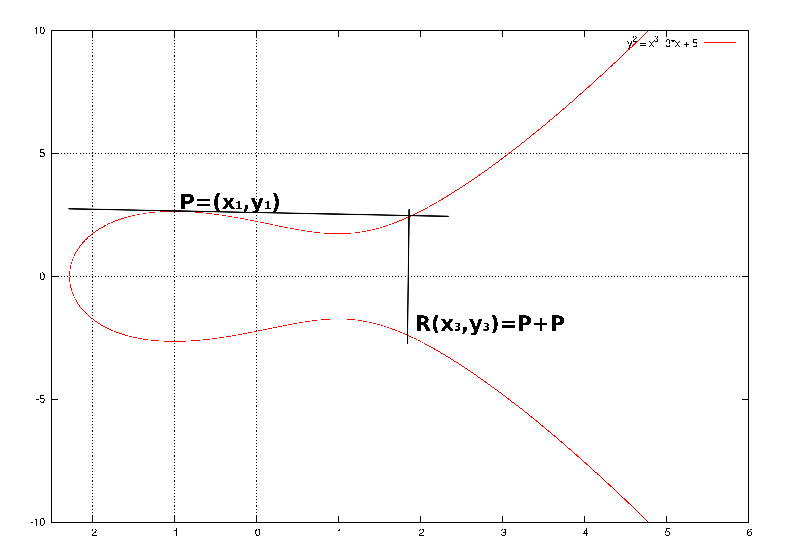
\includegraphics[width=0.6\linewidth]{figures/doubleEC.eps}
              \caption{Doubling a point}
              \label{fig:ecDouble}
          \end{figure}
%      \end{minipage}
%  \end{minipage}
% Formulae to calculate x- and y-coordinates for the resulting points
% for point addition $R=P+Q$ and point doubling $R=P+P$ are shown in equations \ref{adding} and \ref{doubling} respectively:
% 
% 
% \begin{align}\label{doubling}
%  x_3 = (\frac{3x_1^2 +a}{2y_1})^2 - 2x_1, y_3=\frac{3x_1^2+a}{2y_1}(x_1-x_3)-y_1
% \end{align}
Multiplication is defined as successive addition of a point to it self in the way
\begin{center}
 $kP = \underbrace{P+P+...+P}_{k-times}$
\end{center}


\subsubsection{\gls{ecdlp}}\label{ecdp}

Based on this group operations, the \gls{ecdlp} \cite{ecdlp} can be defined as following: given an \gls{ec} $E$ over the finite field $\mathcal{F}_p$, $P$ of order $n$ of this curve 
and a point $Q$, find the integer $k$ s.t. $Q = kP$. $k$ is called the discrete logarithm of $Q$ to the base $P$.
\\
\\
To find $k$, the most naive algorithm trying all possible numbers will terminate after $\frac{n}{2}$ on average. In contrast, the running time of the best known attack is bounded by 
$\sqrt{p}$, where $p$ is the largest prime divisor of $n$. Therefore, such an attack is infeasible for properly chosen \gls{ec} parameters.
%Additionally to the CIA - triad, sometimes two more concepts are used in the security field: \textbf{Authenticity} is tied to integrity and ensures the property
%of being genuine, while \textbf{Accountability} allows to link actions performed on a system uniquely to the entity responsible for them.
